 \subsection{An User visualizes his History data, through a customized research}
 
The user can access to its past data stored in the system, specifying the interval time of interest or the location in which the data were collected. If the user does not insert any preference, are shown all the available data, and the user can reads them performing a manual research.
The data can be visualized ordered by time or by location (e.g. the health data collected when the user were in the city of Milan).




\begin{table}[H]
	\centering
    
    \begin{tabular}{|p{3.5cm}|p{10.3cm}|}
    
    \hline
    \textbf{\large{Actors}}  			& \tabitem  User  				\\
    				 	

    \hline
    \textbf{\large{Goals}} 				&\ref{goal:user3};
              \\
     \hline
    \textbf{\large{Enter Condition}} 
    & The user should be logged in the Data4Help System	
           \\
    
    \hline
    \textbf{\large{Events Flow}}		& \begin{enumerate}[leftmargin=0.5cm]
                                          	\item The \emph{User}  presses the "History" button.
                                            \item The \emph{System} asks to specify what kind of parameters he wants to see
                                            \item The \emph{User} specifies the parameters that wants to receive
                              \item The \emph{User} can specify the time or the location range 
                            \item The \emph{System} retrieves the informations requested from the database
                              \item  The  \emph{System} orders the data by time and location
                                            \item The \emph{System} shows the data to the user.The data can be visualized either in time order or in location order.
            \item The \emph{User} selects the visualization order
            
           \item In case of localization data, The \emph{User} 
           can views them more in detail on an interactive map pressing on the map button.            \end{enumerate}
    										\\
    \hline
    \textbf{\large{Exit Condition}} 	& The user can examine the requested data. \\
    
    \hline
    \textbf{\large{Exception}} 			& The requested data does not exist in the database . \newline
    In this case the system shows an error message and invites the user to insert consistent preferences.\\
    
    \hline
    
    
    \end{tabular}
	
\end{table}
\begin{figure}[H]
    \centering
    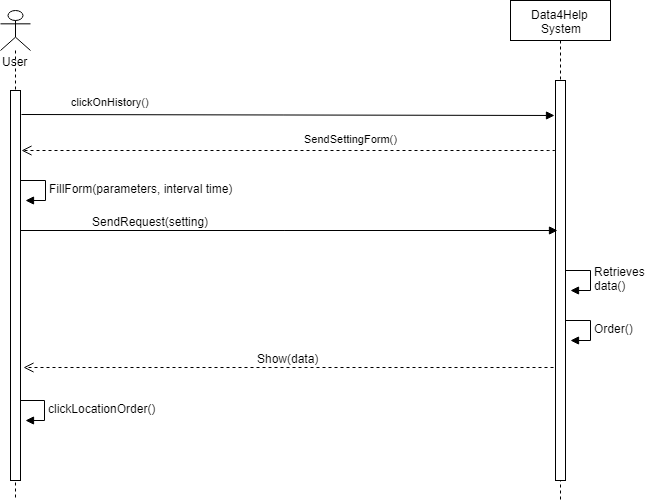
\includegraphics[scale=0.4]{rasdL/Pictures/history.png}
     \caption{In this Use case we suppose that the user performs a history search on his data specifying an interval time and visualizes them in location order}
    
\end{figure}
